\documentclass{article}

\usepackage{graphicx}
\usepackage{amsmath}
\usepackage{amssymb}
\usepackage{caption}

\renewcommand{\figurename}{Figura}

\begin{document}

\begin{flushleft}
    \LARGE Banjercito \\[6pt]
    \Large Diplomado en Ciencia de Datos
\end{flushleft}

\vfill

\begin{flushleft}
    \LARGE \textbf{Guía de Estudio} \\[12pt]
    \LARGE Evaluación Final \\[24pt]
\end{flushleft}

\vfil

\begin{flushleft}
    Alan Badillo Salas \\[12pt]
    \scriptsize Diciembre 2024 \\[24pt]
\end{flushleft}

\vfill

\section*{Introducción}

El Diplomado en Ciencia de Datos ha llegado a su etapa final, dentro del diplomado hemos aprendido a lo largo de 5 módulos, el uso de las herramientas más importantes usadas en el campo de la ciencia de datos. En el primer módulo hemos introducido el análisis financiero a través de Excel, Power BI y Python, en el segundo módulo hemos reunido los conceptos más importantes de probabilidad y estadística, en el tercer módulo hemos trabajado más a detalle con las librerías de Numpy y Pandas y el flujo de la ciencia de datos, en el cuarto módulo hemos aprendido las tres piezas fundamentales del Machine Learning, que son la Regresión, la Clasificación y la Clusterización, así como la simulación estadística y probabilística, finalmente, en el quinto módulo hemos generalizado todos los modelos, para que una Red Neuronal pueda hacer los pronósticos generalizados a través del Deep Learning.
\\[12pt]
En esta guía repasaremos los fundamentos de cada módulo, a través de preguntas y reactivos similares a los de la evaluación final del diplomado, cubriendo los conceptos vistos en cada módulo y detallando su solución. Comprender esta guía debería ser suficiente para tener un buen desempeño como Científico de Datos y estar preparado para problemas del mercado actual y aplicaciones reales en la industria y el gobierno.

\clearpage

\section*{Módulo I | Introducción a Python con Finanzas}

\subsection*{Problema 1 | Uso de Excel}

Una empresa financiera posee una tabla con los montos de créditos que ha aprobado a sus clientes. La tabla posee el género de cada cliente y se desea calcular el monto total de los créditos aprobados para hombres y mujeres.
\\[12pt]
En la Figura \ref{fig:p101-1} se muestra la tabla con el cliente, género, crédito y monto aprobado.
\begin{figure}[!h]
    \centering
    \begin{minipage}{\textwidth}
        \centering
        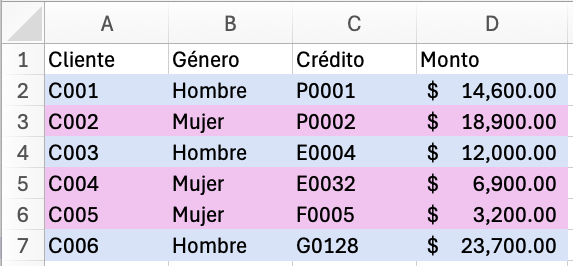
\includegraphics[width=\textwidth]{figures/p101-1.png}
    \end{minipage}
    % \hfill
    % \begin{minipage}{0.4\textwidth}
    %     \centering
    %     \includegraphics[width=\textwidth]{figures/d001.png}
    % \end{minipage}
    % \hfill
    \captionsetup{width=0.9\textwidth}
    \caption{Créditos aprobados a clientes por género}
    \label{fig:p101-1}
\end{figure}
\\
(a) Calcule la suma suma de los montos para hombres y la suma de montos para mujeres usando la fórmula \texttt{=SUMA.SI(RANGO CRITERIO, CRITERIO, RANGO SUMA)}.
\\[6pt]
(b) Calcule la suma suma de los montos para hombres y la suma de montos para mujeres usando la fórmula \texttt{=SUMA(FILTRAR(RANGO SUMA, RANGO INCLUIR))}.

\clearpage

\subsubsection*{Solución al Problema 1}

Para el inciso (a) utilizamos las fórmulas
\\[12pt]
\texttt{=SUMAR.SI(B2:B7,"HOMBRE",D2:D7)}
\\[0pt]
\texttt{=SUMAR.SI(B2:B7,"MUJER",D2:D7)}
\begin{figure}[!h]
    \centering
    \begin{minipage}{\textwidth}
        \centering
        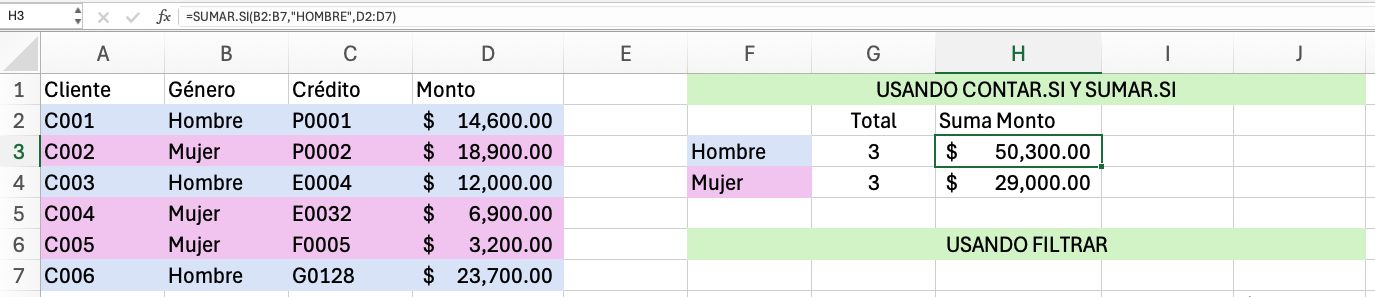
\includegraphics[width=\textwidth]{figures/s101-1a1.png}
    \end{minipage}
    \hfill
    \begin{minipage}{\textwidth}
        \centering
        
\includegraphics[width=\textwidth]{figures/s101-1a2.png}
    \end{minipage}
    \captionsetup{width=0.9\textwidth}
    \caption{Solución al Problema 1 inciso (a)}
    \label{fig:s101-1a}
\end{figure}

\noindent
Para el inciso (b) utilizamos las fórmulas
\\[12pt]
\texttt{=SUMA(FILTRAR(D2:D7,B2:B7="HOMBRE"))}
\\[0pt]
\texttt{=SUMA(FILTRAR(D2:D7,B2:B7="MUJER"))}
\begin{figure}[!h]
    \centering
    \begin{minipage}{\textwidth}
        \centering
        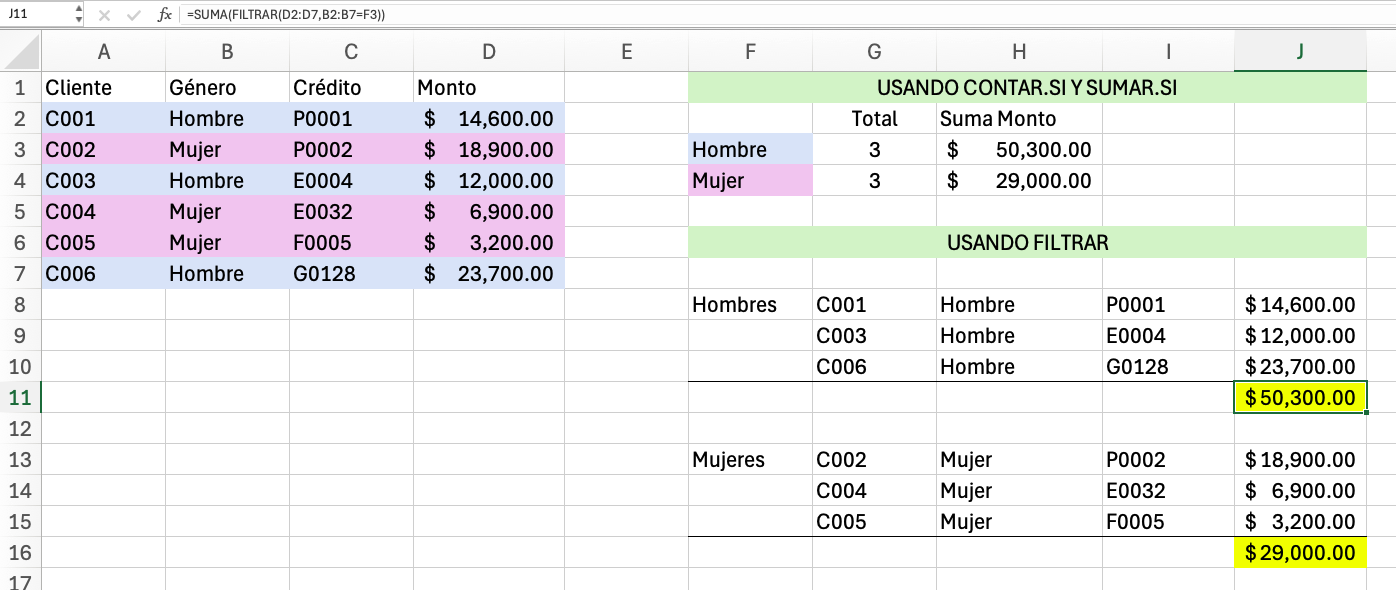
\includegraphics[width=\textwidth]{figures/s101-1b1.png}
    \end{minipage}
    \hfill
    \begin{minipage}{\textwidth}
        \centering
        
\includegraphics[width=\textwidth]{figures/s101-1b2.png}
    \end{minipage}
    \captionsetup{width=0.9\textwidth}
    \caption{Solución al Problema 1 inciso (b)}
    \label{fig:s101-1b}
\end{figure}

\noindent
Nota: Si se utilizamos las fórmulas
\\[12pt]
\texttt{=FILTRAR(A2:D7,B2:B7="HOMBRE")}
\\[0pt]
\texttt{=FILTRAR(A2:D7,B2:B7="HOMBRE")}
\\[12pt]
Se generará la tabla virtual con todos los créditos correspondientes a las filas de los hombres o de las mujeres.
\begin{figure}[!h]
    \centering
    \begin{minipage}{\textwidth}
        \centering
        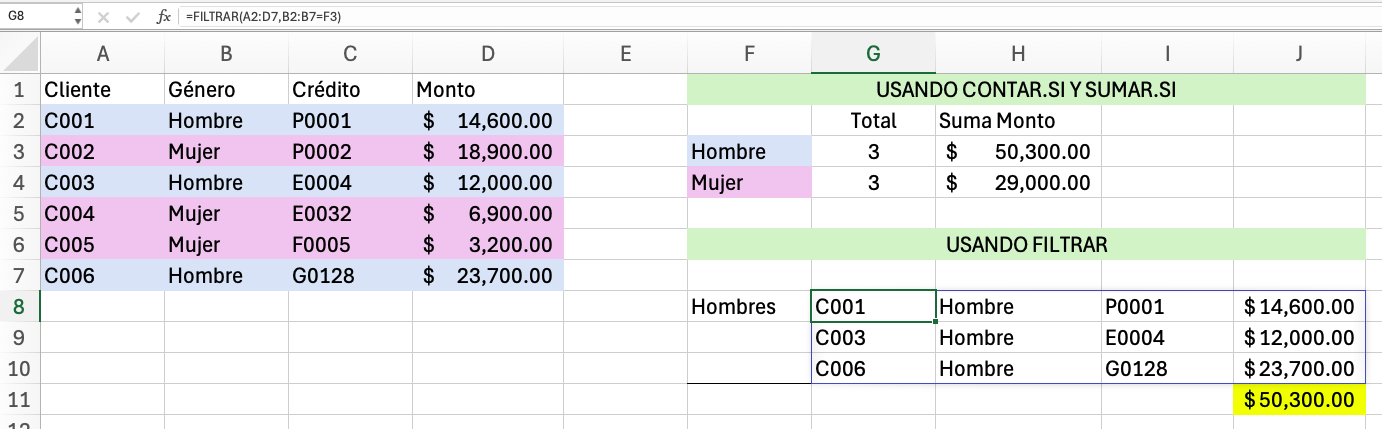
\includegraphics[width=\textwidth]{figures/s101-2.png}
    \end{minipage}
    \hfill
    \begin{minipage}{\textwidth}
        \centering
        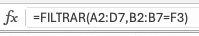
\includegraphics[width=\textwidth]{figures/s101-3.png}
    \end{minipage}
    \hfill
    \begin{minipage}{\textwidth}
        \centering
        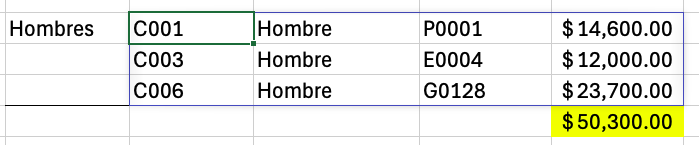
\includegraphics[width=\textwidth]{figures/s101-4.png}
    \end{minipage}
    \captionsetup{width=0.9\textwidth}
    \caption{Tabla virtual generada por FILTRAR (c)}
    \label{fig:s101-c}
\end{figure}

\clearpage

\subsection*{Problema 2 | Uso de Tablas dinámicas en Excel}

Una empresa financiera posee una tabla con los montos de créditos que ha aprobado a sus clientes y su deuda actual. La tabla posee el género de cada cliente y se desea calcular la deuda total y deuda promedio.
\\[12pt]
En la Figura \ref{fig:p102} se muestra la tabla con el cliente, género, crédito, monto aprobado y deuda actual.
\begin{figure}[!h]
    \centering
    \begin{minipage}{\textwidth}
        \centering
        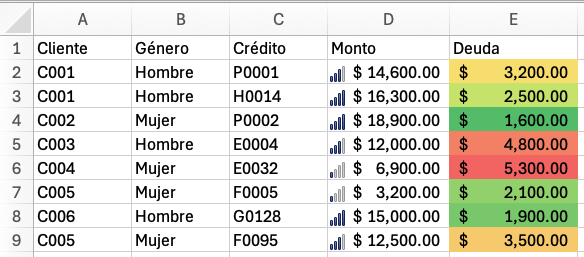
\includegraphics[width=\textwidth]{figures/p102.png}
    \end{minipage}
    % \hfill
    % \begin{minipage}{0.4\textwidth}
    %     \centering
    %     \includegraphics[width=\textwidth]{figures/d001.png}
    % \end{minipage}
    % \hfill
    \captionsetup{width=0.9\textwidth}
    \caption{Créditos aprobados con deuda actual a clientes por género}
    \label{fig:p102}
\end{figure}
\\
(a) Crea una tabla dinámica de \texttt{A1:E9}.
\\[6pt]
(b) Segmenta las filas por Género y luego por Cliente.
\\[6pt]
(c) Cuenta el número de Créditos en valores.
\\[6pt]
(d) Calcula la suma del Monto en valores.
\\[6pt]
(e) Calcula la suma de la Deuda en valores.
\\[6pt]
(f) Calcula el promedio del Monto en valores.
\\[6pt]
(g) Calcula el promedio de la Deuda en valores.
\\[6pt]
(h) ¿Quién es el cliente de mayor deuda?
\\[6pt]
(i) ¿Quién es el cliente al que se le ha prestado más en promedio?
\\[6pt]
(j) ¿Quién es el cliente hombre con mayor deuda promedio?
\\[6pt]
(k) ¿Es significativamente distinta la deuda entre hombres y mujeres?
\\[6pt]
(l) ¿Cuánto se ha recuperado en total de todos los créditos?

\clearpage

\subsubsection*{Solución al Problema 2}

Para el inciso (a) creamos la tabla dinámica para el rango \texttt{A1:E9} y la insertamos en una celda de la misma hoja.
\begin{figure}[!h]
    \centering
    \begin{minipage}{\textwidth}
        \centering
        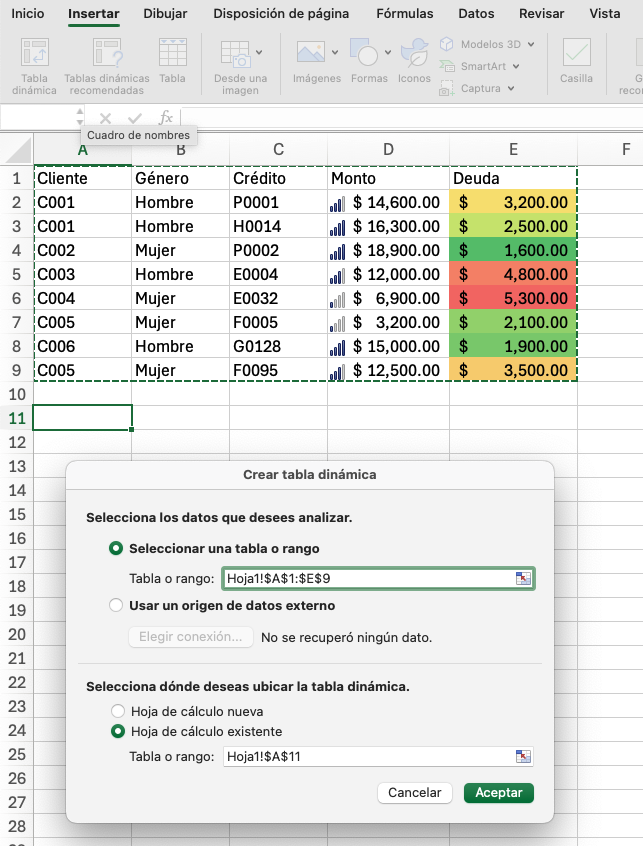
\includegraphics[width=\textwidth]{figures/s102-1.png}
    \end{minipage}
    \captionsetup{width=0.9\textwidth}
    \caption{Solución al Problema 2 inciso (a)}
    \label{fig:s102-1}
\end{figure}

\noindent
Para el inciso (b) arrastramos los campos del género y cliente a las filas
\begin{figure}[!h]
    \centering
    \begin{minipage}{\textwidth}
        \centering
        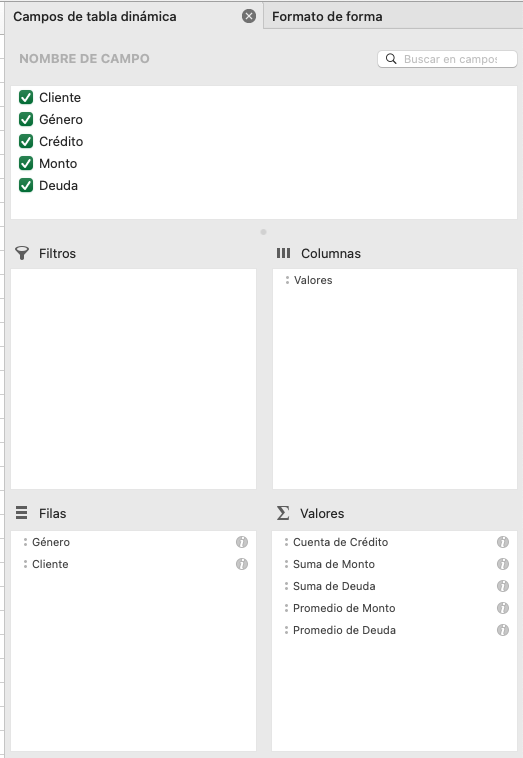
\includegraphics[width=\textwidth]{figures/s102-2.png}
    \end{minipage}
    \captionsetup{width=0.9\textwidth}
    \caption{Solución al Problema 2 inciso (b)}
    \label{fig:s102-2}
\end{figure}

\noindent
Para el inciso (c), (d), (e), (f), (g) arrastramos los campos como valores y configuramos cada campo si es recuento, suma o promedio
\begin{figure}[!h]
    \centering
    \begin{minipage}{\textwidth}
        \centering
        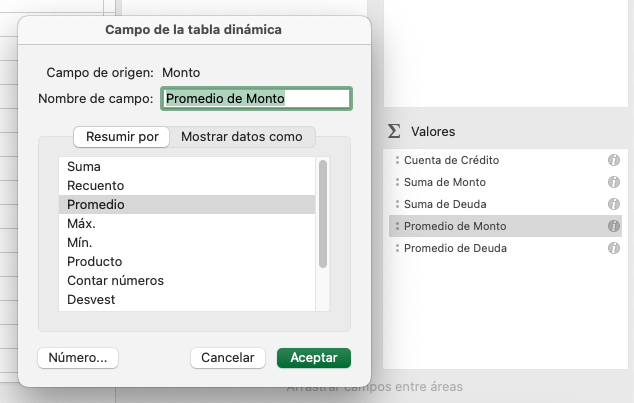
\includegraphics[width=\textwidth]{figures/s102-3.png}
    \end{minipage}
    \captionsetup{width=0.9\textwidth}
    \caption{Solución al Problema 2 incisos (c), (d), (e), (f), (g)}
    \label{fig:s102-3}
\end{figure}

\noindent
Para el inciso (h), (i), (j), (k), (l) observamos los valores en la tabla dinámica
\begin{figure}[!h]
    \centering
    \begin{minipage}{\textwidth}
        \centering
        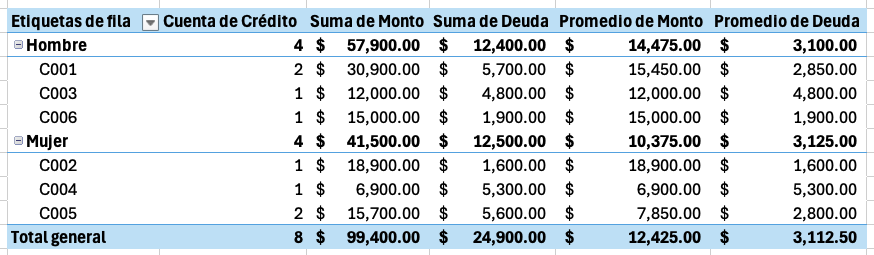
\includegraphics[width=\textwidth]{figures/s102-4.png}
    \end{minipage}
    \captionsetup{width=0.9\textwidth}
    \caption{Solución al Problema 2 incisos (h), (i), (j), (k), (l)}
    \label{fig:s102-4}
\end{figure}

\noindent
Respuestas: (h) \textbf{C001 \$5,700}, (i) \textbf{C002 \$18,900}, (j) \textbf{C003 \$4,800}, (k) \textbf{No, la diferencia es de \$100 menor al 1\% de diferencia}, (l) \textbf{\$74,500 = \$99,400 - \$24,900}.

\clearpage

\subsection*{Problema 3 | Uso de Power BI}

Una empresa financiera posee una tabla con los préstamos que ha aprobado a sus clientes indicando el monto, el estado y el valor. En cada préstamo se reporta el estado de sobre lo que se ha pagado del préstamo, lo que se debió haber cubierto actualmente (deuda) y lo que se debería cubrir en el futuro (pendiente). La financiera requiere una tabla que resuma de cada cliente sus préstamos y en cada préstamo se desglose la suma de cuánto adeuda, cuánto ha pagado y cuánto está pendiente, así como el total. También requiere un indicador que muestre la diferencia entre la suma del monto del préstamo y el valor del monto pagado, para saber cuánto se adeuda en total del préstamo, igualmente desglosado por cliente y préstamo. Finalmente la financiera requiere dos reportes visuales, un anillo que muestre el estado de los préstamos (pagado, pendiente y deuda) segmentado por cliente. Y un esquema jerárquico que permita desglosar el valor del préstamo por su estado, cliente y número de préstamo.
\\[12pt]
En la Figura \ref{fig:p103} se muestra la tabla de préstamos, con la columna del cliente, el número de préstamo, el monto, el estado (pagado, deuda, pendiente) y el valor asociado al estado.
\begin{figure}[!h]
    \centering
    \begin{minipage}{\textwidth}
        \centering
        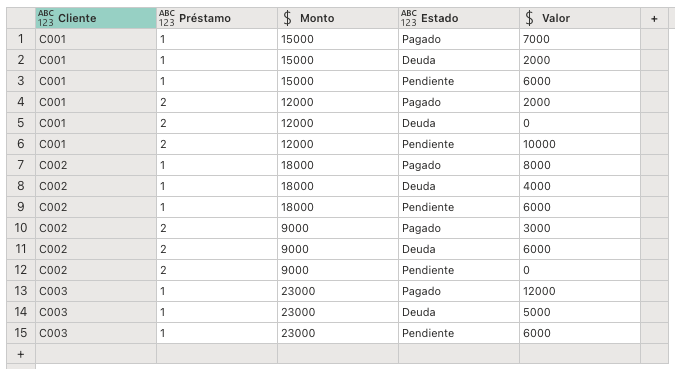
\includegraphics[width=\textwidth]{figures/p103.png}
    \end{minipage}
    \captionsetup{width=0.9\textwidth}
    \caption{Préstamos aprobados a clientes desglosado por cliente, número de préstamo, estado (pagado, deuda y pendiente) y valor asociado al estado}
    \label{fig:p103}
\end{figure}
\\

\break
\noindent
(a) Crea una matriz que reporte las filas para el cliente y número de préstamo en ese orden, el estado como columna y la suma del valor en los valores.
\\[6pt]
(b) En el modelo de datos crea una nueva medida con la fórmula
\\[6pt]
\texttt{Diferencia = SUM(P103[Monto])-SUM(P103[Valor])} 
\\[6pt]
para reportar la diferencia entre la suma del monto menos la suma del valor asociado al estado. Donde \textit{P103} es el nombre de la tabla creada al inicio.
\\[6pt]
(c) Crea una matriz que reporte las filas para el cliente y número de préstamo en ese orden, el estado como columna y la suma del monto, suma del valor y suma de diferencia en los valores en ese orden. Reporta solo el estado Pagado en los filtros del objeto visual.
\\[6pt]
(d) Crea una gráfica de anillo cuya leyenda este dada por el estado del préstamo, en valores reporte la suma del valor asociado al estado, y en detalles segmente al cliente.
\\[6pt]
(e) Crea un esquema jerárquico para analizar la suma del valor valor asociado al estado, explicado por el estado del préstamo, el cliente y el número de préstamo en ese orden.
\\[6pt]
(f) De la matriz del inciso (a) responde si cada desglose corresponde al monto reportado en cada préstamo.
\\[6pt]
(g) De la matriz del inciso (b) responde cuál el es el préstamo con menor deuda total y usando el inciso (a) cómo es su deuda respecto al préstamo.
\\[6pt]
(h) Del anillo identifica al cliente de mayor deuda y el cliente con mayor valor pendiente.
\\[6pt]
(i) Del esquema jerárquico identifica al cliente de mayor deuda y el número de préstamo de mayor deuda para ese cliente.

\clearpage

\subsubsection*{Solución al Problema 3}

Para el inciso (a) creamos una matriz que reporte las filas para el cliente y número de préstamo en ese orden, el estado como columna y la suma del valor en los valores.
\begin{figure}[!h]
    \centering
    \begin{minipage}{\textwidth}
        \centering
        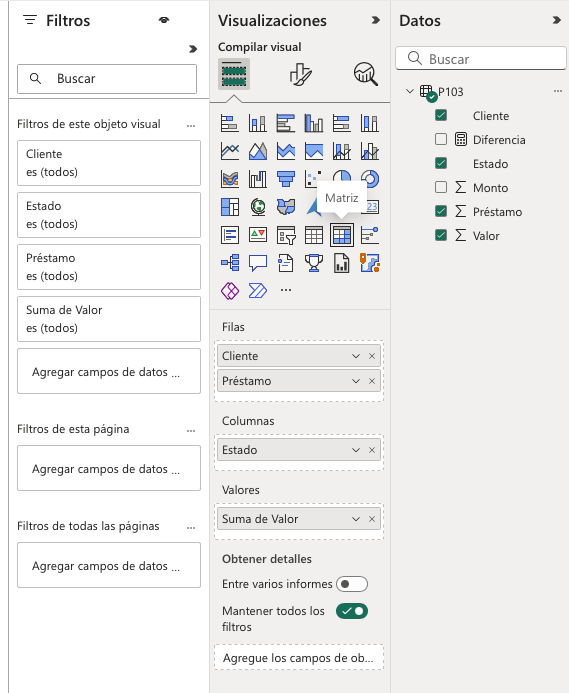
\includegraphics[width=0.7\textwidth]{figures/s103a-1.png}
    \end{minipage}
    \hfill
    \begin{minipage}{\textwidth}
        \centering
        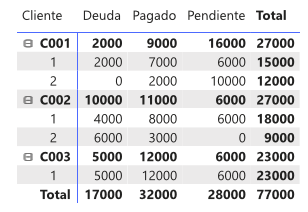
\includegraphics[width=0.7\textwidth]{figures/s103a-2.png}
    \end{minipage}
    \captionsetup{width=0.9\textwidth}
    \caption{Solución al Problema 3 inciso (a)}
    \label{fig:s103a}
\end{figure}

\noindent
Para el inciso (b) abrimos el modelo de datos y dentro del modelo de datos creamos una nueva medida con la fórmula para calcular la diferencia.
\begin{figure}[!h]
    \centering
    \begin{minipage}{\textwidth}
        \centering
        
\includegraphics[width=\textwidth]{figures/s103b-1.png}
    \end{minipage}
    \hfill
    \begin{minipage}{\textwidth}
        \centering
        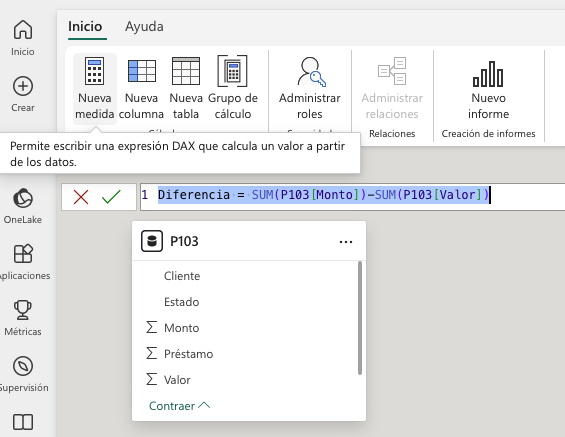
\includegraphics[width=\textwidth]{figures/s103b-2.png}
    \end{minipage}
    \hfill
    \begin{minipage}{\textwidth}
        \centering
        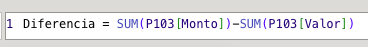
\includegraphics[width=\textwidth]{figures/s103b-3.png}
    \end{minipage}
    \captionsetup{width=0.9\textwidth}
    \caption{Solución al Problema 3 inciso (b)}
    \label{fig:s103b}
\end{figure}

\break
\noindent
Para el inciso (c) creamos una matriz que reporte las filas para el cliente y número de préstamo en ese orden, el estado como columna y la suma del monto, suma del valor y suma de diferencia en los valores en ese orden. Reporta solo el estado Pagado en los filtros del objeto visual.
\begin{figure}[!h]
    \centering
    \begin{minipage}{\textwidth}
        \centering
        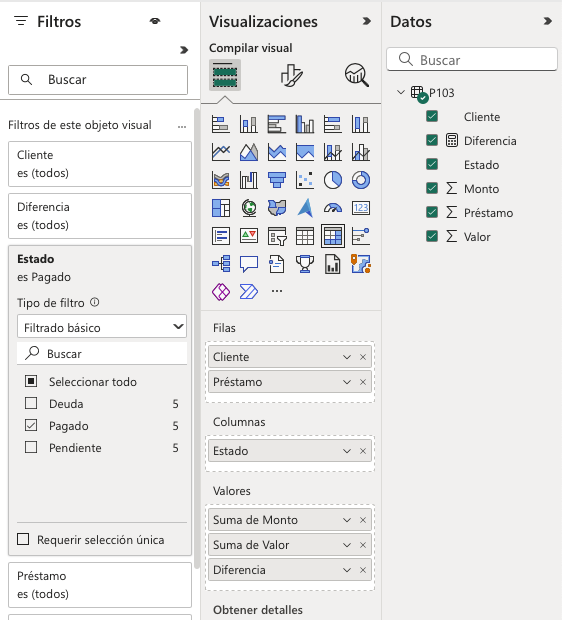
\includegraphics[width=0.9\textwidth]{figures/s103c-1.png}
    \end{minipage}
    \hfill
    \begin{minipage}{\textwidth}
        \centering
        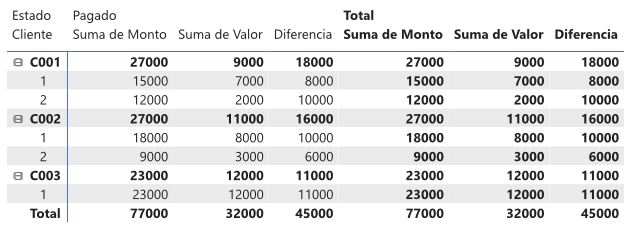
\includegraphics[width=0.9\textwidth]{figures/s103c-2.png}
    \end{minipage}
    \captionsetup{width=0.9\textwidth}
    \caption{Solución al Problema 3 inciso (c)}
    \label{fig:s103c}
\end{figure}

\noindent
Para el inciso (d) creamos una gráfica de anillo cuya leyenda este dada por el estado del préstamo, en valores reporte la suma del valor asociado al estado, y en detalles segmente al cliente.
\begin{figure}[!h]
    \centering
    \begin{minipage}{\textwidth}
        \centering
        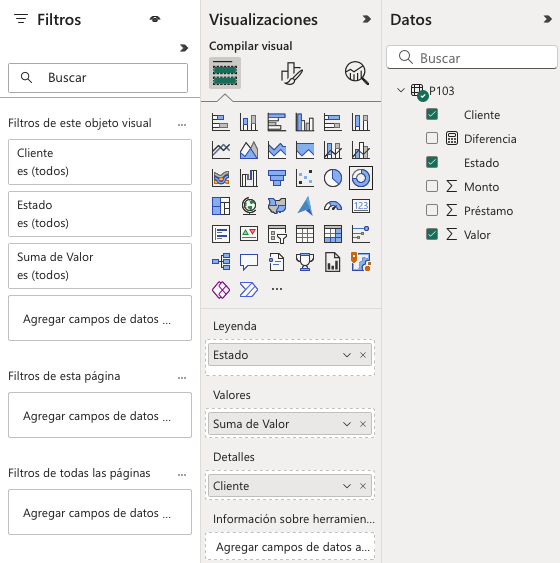
\includegraphics[width=0.8\textwidth]{figures/s103d-1.png}
    \end{minipage}
    \hfill
    \begin{minipage}{\textwidth}
        \centering
        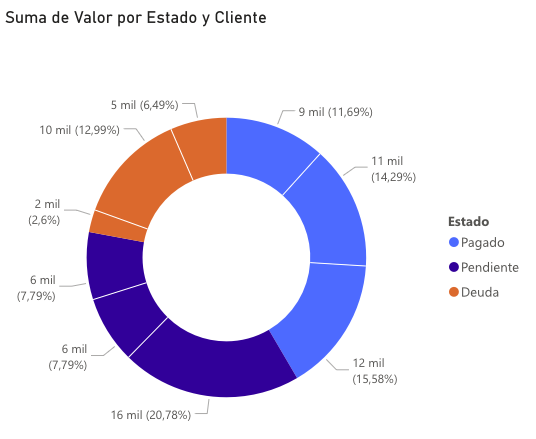
\includegraphics[width=0.7\textwidth]{figures/s103d-2.png}
    \end{minipage}
    \captionsetup{width=0.9\textwidth}
    \caption{Solución al Problema 3 inciso (d)}
    \label{fig:s103d}
\end{figure}

\noindent
Para el inciso (e) creamos un esquema jerárquico para analizar la suma del valor valor asociado al estado, explicado por el estado del préstamo, el cliente y el número de préstamo en ese orden.
\begin{figure}[!h]
    \centering
    \begin{minipage}{\textwidth}
        \centering
        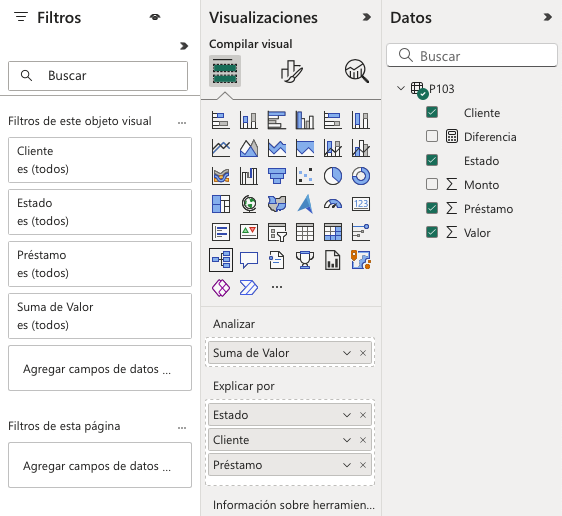
\includegraphics[width=0.9\textwidth]{figures/s103e-1.png}
    \end{minipage}
    \hfill
    \begin{minipage}{\textwidth}
        \centering
        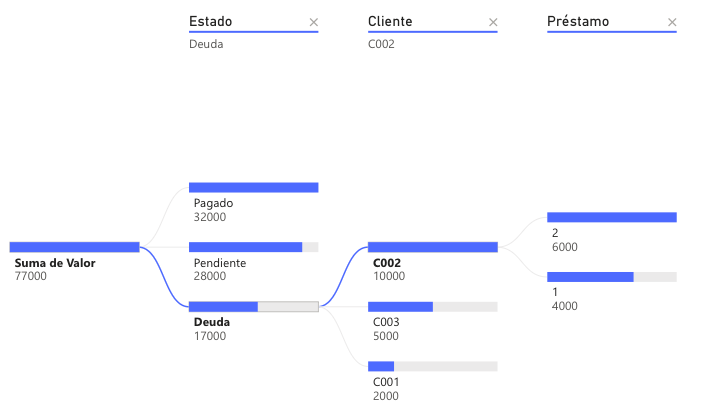
\includegraphics[width=0.9\textwidth]{figures/s103e-2.png}
    \end{minipage}
    \captionsetup{width=0.9\textwidth}
    \caption{Solución al Problema 3 inciso (e)}
    \label{fig:s103e}
\end{figure}

\noindent
Para los otros incisos las respuestas son: (f) Sí, la suma de montos en cada préstamo coincide con la suma de su deuda, lo pagado y lo pendiente. (g) Para el cliente \textit{C002} en el préstamo número \textit{2} la diferencia total es de \textbf{\$6,000} y es el préstamo de menor deuda, ya que lo pendiente para ese préstamo es de \textbf{\$0}, sin embargo, respecto a los otros préstamos es el de mayor deuda. (h) \textbf{C002 \$10,000 12.99\%} es el cliente de mayor deuda y \textbf{C001 \$16,000 20.78\%} es el cliente de mayor valor pendiente. (i) \textbf{C002 \$10,000 2 \$10,000} es el cliente de mayor deuda, con su préstamo número dos.

\clearpage

\subsection*{Problema 4 | Uso de Python}

Un banco ha decidido usar Python en un ambiente controlado para poder hacer operaciones y cálculos de riesgo, para ello ha instalado un ambiente virtual cerrado en computadoras sin acceso a internet para que no se filtren los conjuntos de datos utilizados, ni los reportes generados.
\\[12pt]
El banco comenzará por automatizar una serie de funciones útiles que pueda aplicar para cálculos simples, para de esta forma crear una metodología de trabajo cuando deseen incrementar el volumen de las operaciones.
\\[12pt]
Para ello, el banco requiere que se generen los siguientes reportes automatizados para saber que todo está funcionando correctamente.
\\[12pt]
Implementa las funciones que se detallan a continuación y resuelve los incisos siguietes. Completa el código que haga falta para que las funciones operen correctamente siguiendo las pistas de los comentarios
\scriptsize
\begin{verbatim}
def reporteTitulo(codigo, leyenda):
    print(f"Banco Nacional - Reporte {codigo} / {leyenda}")

def reporteCorte(codigo, leyenda):
    print(f"-------------- {codigo} / {leyenda} --------------")

def reporteFin(codigo, leyenda):
    print(f"-------------- {codigo} / {leyenda} --------------")

def reporteBalanceDiaInicio(valance):
    reporteTitulo("BIN", "Balance al Inicio del Día")
    print(f"$ {valance:.2f}")
    reporteFin("BIN", "Balance al Inicio del Día")

def reporteBalanceDiaFin(valance):
    reporteTitulo("B-OUT", "Balance al Final del Día")
    print(f"$ {valance:.2f}")
    reporteFin("B-OUT", "Balance al Final del Día")

def reporteTotalOperacionesDia(numOperaciones):
    reporteTitulo("T-OP", "Total de Operaciones del Día")
    # Imprime el número de operaciones
    reporteFin("T-OP", "Total de Operaciones del Día")

def reporteTotalOperacionesRelativasMes(numOperacionesDia, numOperacionesMes):
    reporteTitulo("T-OR", "Tasa de Operaciones del día respecto al mes")
    tasa = 100 * numOperacionesDia / numOperacionesMes
    # Imprime el número de operaciones del dia
    # luego una diagonal y el número de operaciones del mes
    # Haz un corte del reporte
    # Imprime la tasa de operaciones del día respecto al mes a un dígito
    # Ejemplo: 41/200 (20.5%)
    reporteFin("T-OR", "Tasa de Operaciones del día respecto al mes")
\end{verbatim}
\hfill
\normalsize

\noindent
(a) Reporta el balance de inicio del día con \textbf{\$ 185,000.32}
\\[6pt]
(b) Reporta un total de \textbf{247} operaciones del día
\\[6pt]
(c) Reporta un total de \textbf{247} de \textbf{192,316} operaciones relativas del mes
\\[6pt]
(d) Reporta el balance de fin del día con \textbf{\$ 232,827.71}
\\[6pt]

\subsection*{Problema 5 | Interés Simple}

\subsection*{Problema 6 | Interés Compuesto}

\subsection*{Problema 7 | Tasa de Interés Variable}

\subsection*{Problema 8 | Tabla de Amortización Simple}

\subsection*{Problema 9 | Interés Simple Futuro}

\subsection*{Problema 10 | Punto de Liquidación}

\clearpage

\section*{Módulo II | Estadística y Probabilidad con Python}

\subsection*{Problema 1 | Probabilidad de un Evento Simple}

\subsection*{Problema 2 | Tabla conjunta de Dos Eventos}

\subsection*{Problema 3 | Probabilidad Conjunta de Dos Eventos}

\subsection*{Problema 4 | Probabilidad Condicional de Dos Eventos}

\subsection*{Problema 5 | Probabilidad Conjunta de Tres Eventos}

\subsection*{Problema 6 | Probabilidad Condicional de Tres Eventos}

\subsection*{Problema 7 | Estadísticos Principales de Un Eje}

\subsection*{Problema 8 | Estadísticos Principales de Dos Ejes }

\subsection*{Problema 9 | Matriz de Correlación entre Tres Ejes}

\subsection*{Problema 10 | Prueba F entre Dos Hipótesis de Un Eje}

\clearpage

\section*{Módulo III | Ciencia de Datos}

\subsection*{Problema 1 | Estructuración de un Dataset en Excel}

\subsection*{Problema 2 | Dataset de indicadores en CSV}

\subsection*{Problema 3 | Adquisición de un CSV en Python}

\subsection*{Problema 4 | Indicadores en Series de Pandas}

\subsection*{Problema 5 | Indicadores en DataFrames de Pandas}

\subsection*{Problema 6 | Filtrar columnas en DataFrames}

\subsection*{Problema 7 | Filtrar filas en DataFrames}

\subsection*{Problema 8 | Agrupación de datos en DataFrames}

\subsection*{Problema 9 | Combinación de datos en DataFrames}

\subsection*{Problema 10 | Viasualización de datos}

\clearpage

\section*{Módulo IV | Machine Learning}

\subsection*{Problema 1 | Aprendizaje Supervisado}

\subsection*{Problema 2 | Regresión Simple}

\subsection*{Problema 3 | Regresión Múltiple}

\subsection*{Problema 4 | Clasificación Simple}

\subsection*{Problema 5 | Clasificación Múltiple}

\subsection*{Problema 6 | Aprendizaje No Supervisado}

\subsection*{Problema 7 | Reducción de Dimensionalidad}

\subsection*{Problema 8 | Matriz de Adyacencia}

\subsection*{Problema 9 | Matriz de Similitud}

\subsection*{Problema 10 | Clusterización}

\clearpage

\section*{Módulo IV | Deep Learning}

\subsection*{Problema 1 | Modelo Generalizado}

\subsection*{Problema 2 | Perceptrón Simple}

\subsection*{Problema 3 | Capa de Perceptrones Múltiples}

\subsection*{Problema 4 | Modelo Secuencial Simple}

\subsection*{Problema 5 | Capas Densas Ocultas}

\subsection*{Problema 6 | Regresión Generalizada}

\subsection*{Problema 7 | Clasificación Generalizada}

\subsection*{Problema 8 | Exportación de una Red Neuronal}

\subsection*{Problema 9 | Importación de una Red Neuronal}

\subsection*{Problema 10 | Predicción y Evaluación}

\end{document}